\chapter{Introduction}
\chaptermark{Introduction}
\label{chapter:introduction}

\epigraph{\textit{IoT without security means Internet of Threats}}{Stéphane Nappo}

\minitoc

%%%%%%%%%%%%%%%%%%%%%%%%%%%%%%%%%%%%%%%%%%%%%%%%%%%%%%%%%%%%%%%%%%%%%%%%%%%%%%%%%%%%%%%%%%%%%%%
\section{Context}
An embedded system is a specialised computing system designed to perform dedicated functions or tasks within a larger mechanical or electrical system. Unlike general-purpose computers, embedded systems are optimised for specific control operations and are typically integrated into the hardware they manage. These systems are characterised by their compact size, low power consumption, and real-time performance constraints. They consist of microcontrollers or microprocessors, along with memory and input/output interfaces, tailored to meet the precise requirements of the application they serve. Embedded systems are ubiquitous in modern technology, powering a wide range of devices from household appliances and medical equipment to industrial machines and automotive systems, ensuring efficiency, reliability, and functionality in their operations.

\begin{figure}[ht]
    \centering
    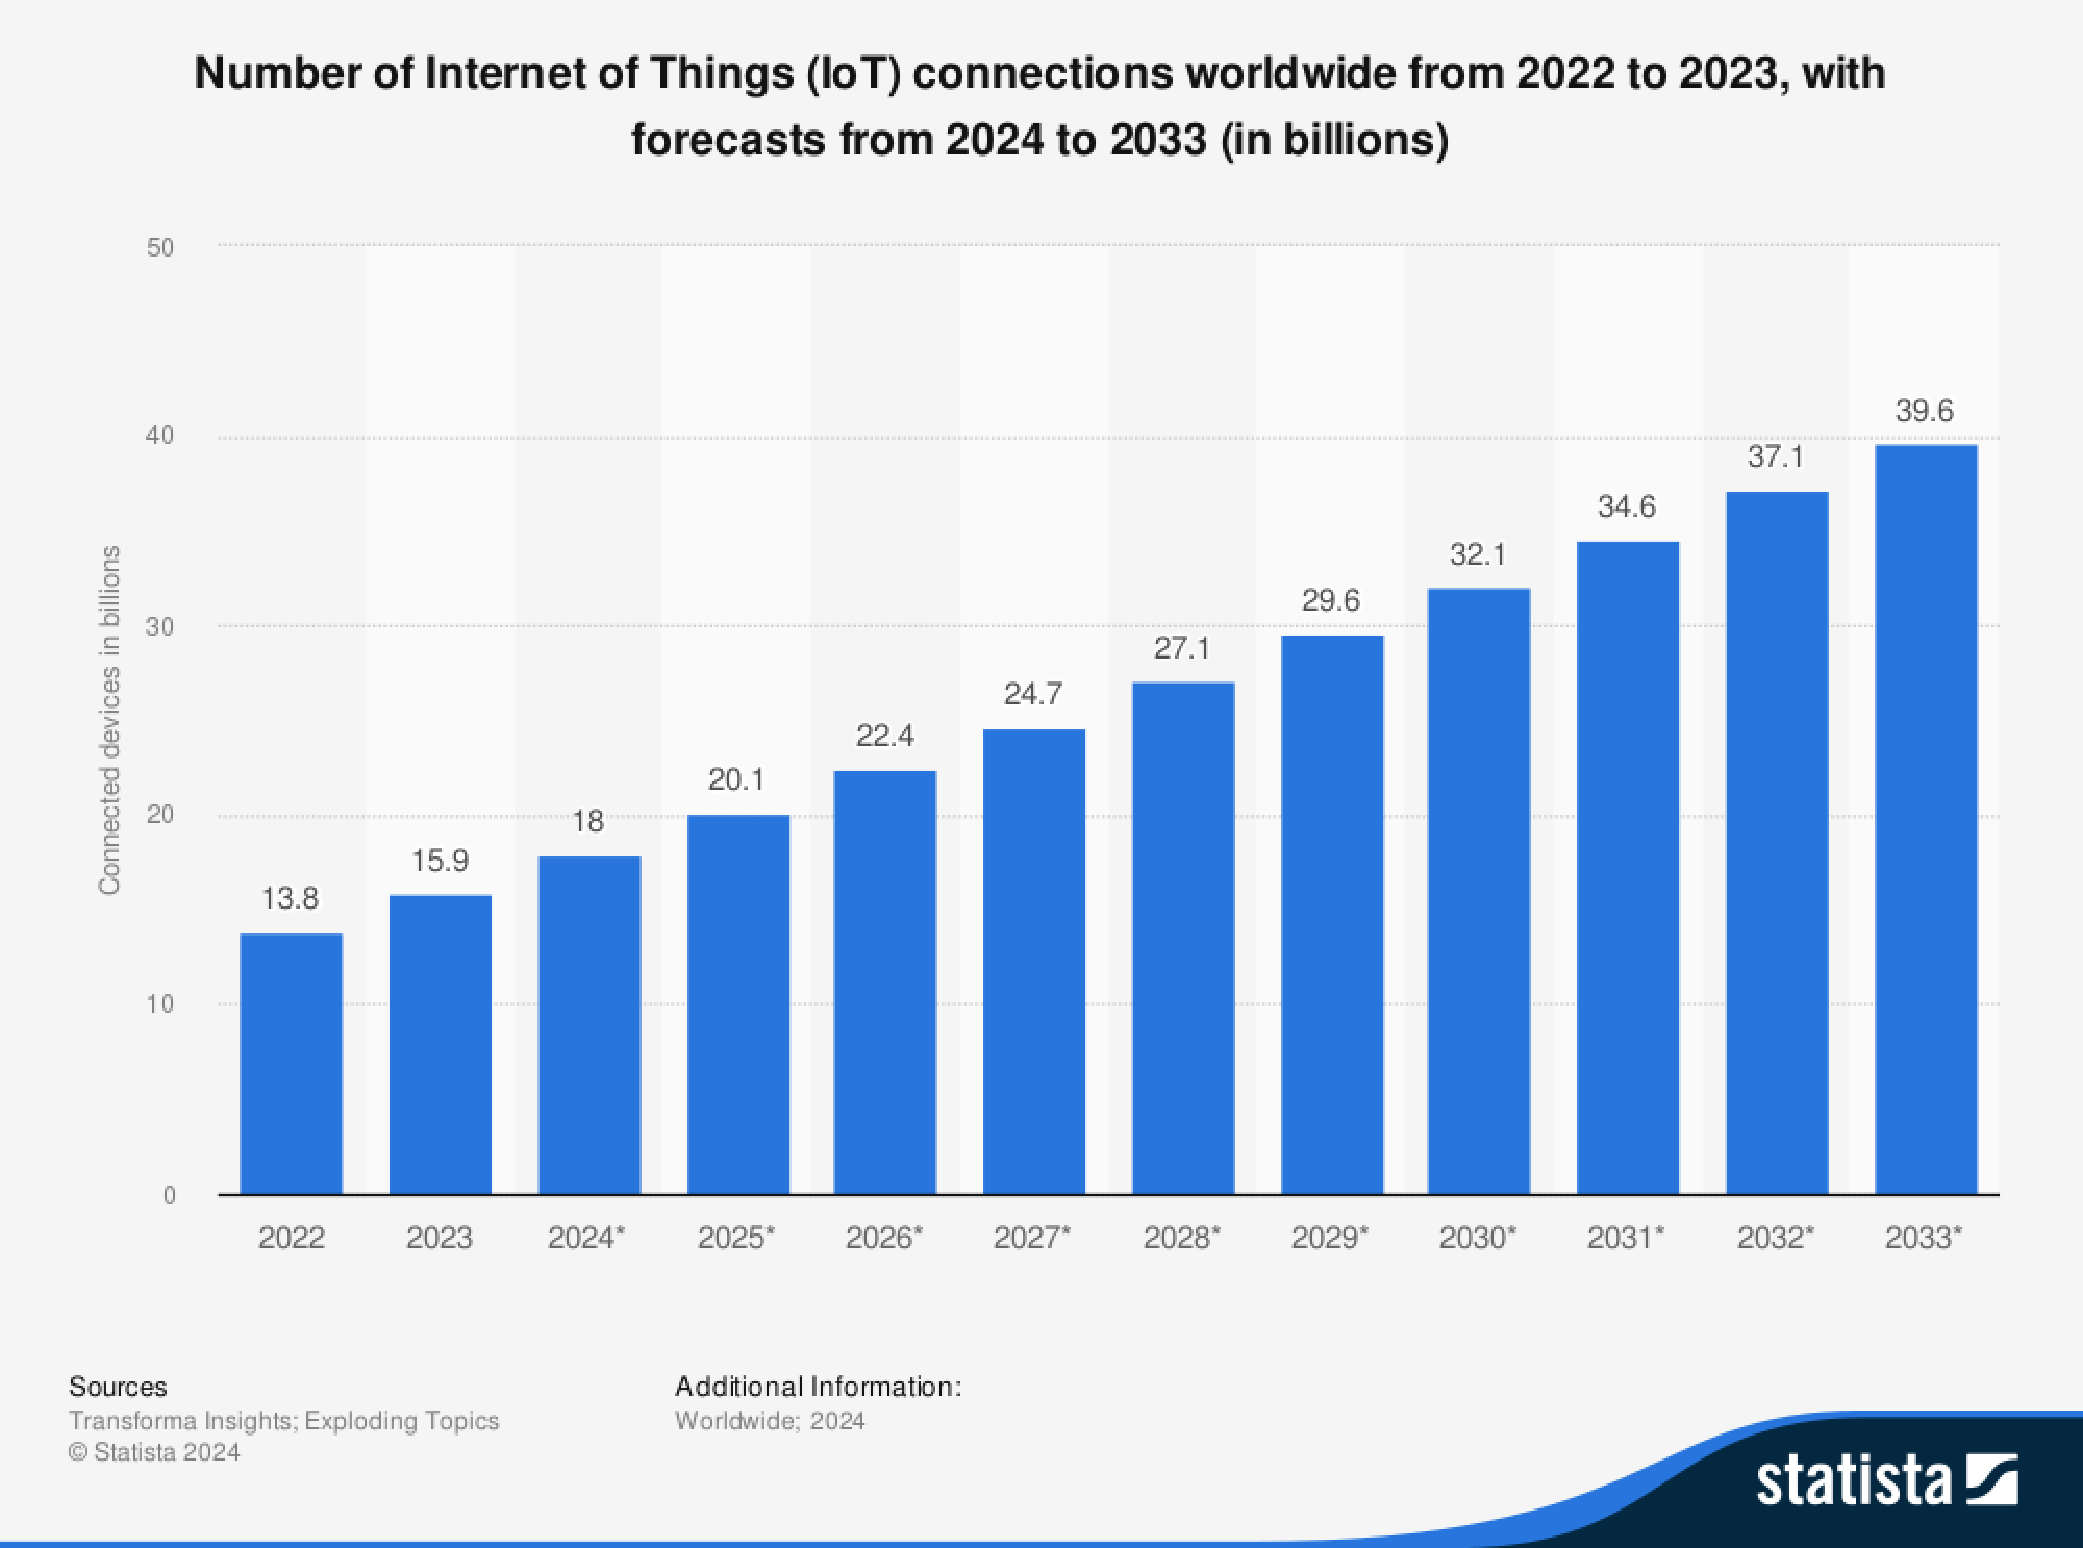
\includegraphics[width=\linewidth, trim={1.25cm 4.75cm 1cm 3.75cm}, clip]{c1_intro/img/iot_forecasts.pdf}
    \caption{Number of IoT (IoT) devices worldwide 2022-2023, with forecasts to 2033 (from~\cite{statista_iot})}
    \label{fig:iot_forecasts}
\end{figure}

The Internet of Things (IoT) has revolutionised the way we interact with technology, enabling seamless connectivity and communication between a myriad of devices. These devices are part of our daily lives, from the connected light bulb to autonomous cars. These devices collect and share data about how they are used and the environment in which they operate.  Immense amounts of data are also being generated by connected cars, production, and transport applications. Today, Industrial IoT (IIoT) represents the largest and fastest-growing volume of data.
To capture data, they rely on sensors embedded in every physical device, such as mobile phones, smartwatches, medical devices (pacemakers, cardiac defibrillators, etc.), but also in recent cars or in agriculture. These sensors generate data that are more or less critical, and as these data exist, they are subjects of cyberattacks.
According to forecasts, the number of IoT devices in use worldwide is estimated to reach approximatively 40 billions in 2033~\cite{statista_iot}, as shown in Figure~\ref{fig:iot_forecasts}, while, today, in 2024, we are around 18 billions. The economic impact of IoT is substantial, with worldwide consumer IoT revenue expected to rise from \$181.5 billion in 2020 to 621.6 billion euros by 2030~\cite{statista_iot_revenu} as shown in Figure~\ref{fig:iot_revenue}.
As IoT continues to expand its reach, the importance of ensuring robust software security in these systems becomes increasingly critical. IoT devices, often characterised by limited resources and large-scale deployment, present unique security and privacy challenges.

\begin{figure}[ht]
    \centering
    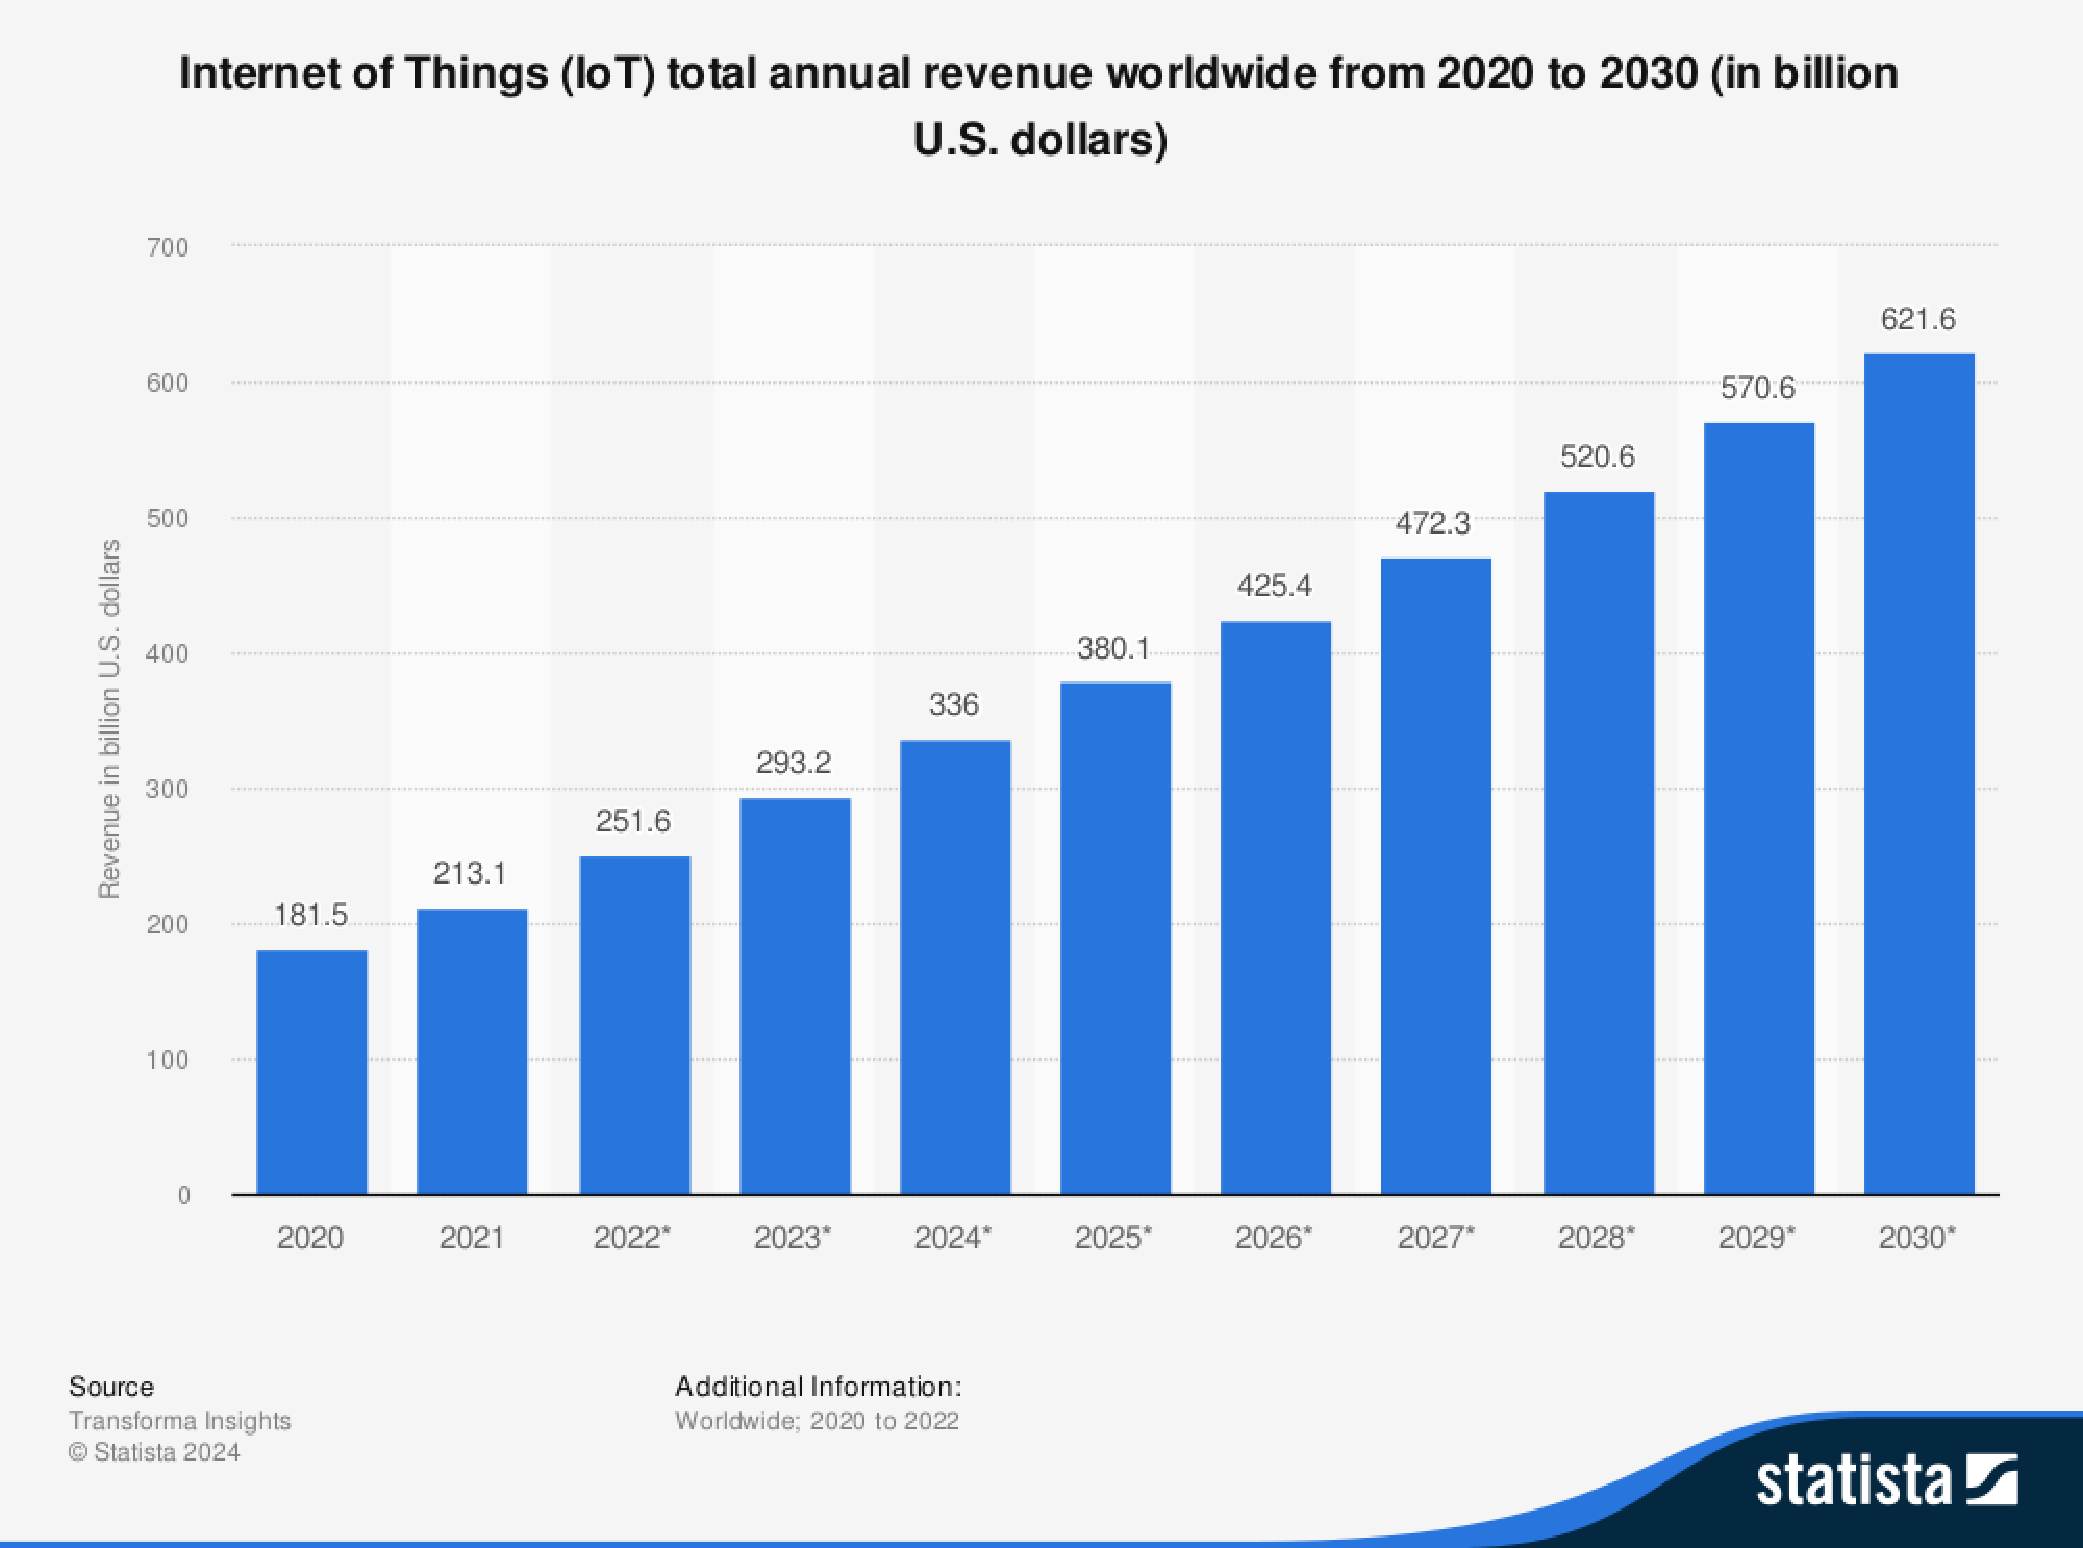
\includegraphics[width=\linewidth, trim={1.25cm 4.75cm 1cm 3.75cm}, clip]{c1_intro/img/iot_revenue.pdf}
    \caption{Internet of Things total annual revenue worldwide from 2020 to 2030 (from~\cite{statista_iot_revenu})}
    \label{fig:iot_revenue}
\end{figure}


Embedded systems, which form the backbone of IoT devices, are increasingly vulnerable to both software and hardware threats, as well as network-based threats, which can lead to data leaks or unauthorised access to essential system components. These systems are frequently deployed in environments where they are exposed to potential adversaries, making them attractive targets for various types of attack~\cite{MW-19-compnet, EAJJMB-22-compscrev}.

Software security is a critical aspect of the development and deployment of software systems, encompassing measures and practices designed to protect applications from malicious attacks, vulnerabilities, and other security risks. It involves the implementation of protocols to ensure the confidentiality, integrity, and availability of software and data. This field addresses a wide range of threats, including but not limited to, code injection, malware, memory overflow attacks, SQL injection, and Cross-site scripting (XSS). Effective software security practices include rigorous code reviews, the use of secure coding standards, regular vulnerability assessments, and the deployment of encryption and authentication mechanisms. As software becomes increasingly integral to various aspects of daily life and business operations, ensuring its security is paramount to safeguarding sensitive information, maintaining user trust, and preventing financial and reputational damage.

Network attacks, such as Distributed Denial of Service (DDoS) attacks, can overwhelm an embedded system's network interface, rendering it inoperative, while man-in-the-middle attacks intercept and potentially alter communication between devices, Internet Protocol spoofing, jamming, and many others. These vulnerabilities can be exploited to leak confidential data, corrupt system functionality, or gain control over critical system operations, underscoring the urgent need for robust security mechanisms in embedded systems.

On the hardware front, physical attacks refer to different techniques and methods aimed at compromising the security of embedded system. These attacks exploit vulnerabilities in the physical layer or implementation of the device’s hardware to delete, modify, gain or prevent access to confidential data.
The most common physical attacks are Side-Channel Attacks (SCA) and Fault Injection Attacks (FIA).

Side-channel attacks~\cite{DM-21-appiot} are passive physical attacks that primarily aim to exploit leakages of information from a device, such as power consumption, electromagnetic emissions, or timing information. By capturing and analysing these side-channel data, attackers can infer sensitive information, such as cryptographic keys~\cite{K-96-crypto}.

Fault injection attacks~\cite{BCNTW-06-procieee, BBKN-12-procieee, YSW-18-hss} are active physical attacks, noninvasive or invasive, transient or permanent, where the attacker intentionally try to change the normal behaviour of a device during program execution by injecting one or more faults, then observing the erroneous behaviour that could be further exploited as a vulnerability. Boneh et al.~\cite{BDL-97-eurocrypt} introduced fault injection attacks. They were able to break some cryptographic protocols by inducing faults into the computations.

In this dissertation, we only study and present fault injection attacks. Nowadays, these attacks are more and more easier to make. For example, NetSPI introduced, in the Black Hat conference in Las Vegas, in August 2024, a new laser hacking device called the RayV Lite~\cite{rayvlite_wired}. The authors, Sam Beaumont and Larry "Patch" Trowell, presented their open-source tool that aims to let anyone achieve laser-based tricks to reverse engineer chips and trigger their vulnerabilities. There are already some tools such as Riscure Laser Station~\cite{riscure_station} who costs between \$10,000 and \$150,000. In the same way as NewAE~\cite{chipwhisperer} with their ChipWhisperer or ChipShouter that allow to realise clock glitching, voltage glitching or even electromagnetic injection at a lower cost and more accessible, RayV Lite allows people to perform laser-based attacks for only \$500 which is more accessible and cheaper than any other tools available.

Many studies have shown the vulnerabilities of critical systems against FIAs.
\cite{LBDP-19-date} demonstrates that it is possible to recover computed secret data using FIA in hidden registers on the RISC-V Rocket processor. 
Electromagnetic fault injection (EMFI) attack can be used to recover an AES key by targeting the cache hierarchy and the MMU, as shown in~\cite{TBELB-21-jce}.
Laser fault injections (LFI) can allow the replay of instructions~\cite{KDD-21-dsd}, that can lead to the overwriting of an entire section of a program.
\cite{TSW-16-fdtc} shows the use of glitch injections on the power supply to control the program counter (PC). Voltage glitches can also lead to glitch TrustZone mechanisms, as shown in~\cite{SMS-23-usenix}.
Finally, authors of~\cite{NSUH-21-tches} have shown that one can combine side-channel attacks (SCA) and FIAs to bypass the PMP mechanism in a RISC-V processor.

Thus, the main challenge of this work is how can we maintain maximum protection against software attacks in the presence of physical attacks ?

%%%%%%%%%%%%%%%%%%%%%%%%%%%%%%%%%%%%%%%%%%%%%%%%%%%%%%%%%%%%%%%%%%%%%%%%%%%%%%%%%%%%%%%%%%%%%%%
\section{Objectives}

In this dissertation, we address a part of the threats that IoT devices faces, with a particular emphasis on security threats affecting the software and hardware layers of a device. The main objective is to provide a robust security mechanism against both software and physical threats where the attacker perform a fault injection attack to bypass a software security mechanism in order to realise a software attack.
We use a security mechanism called Dynamic Information Flow Tracking (DIFT) to protect the system against software attacks. This mechanism is presented in Chapter~\ref{section:ift} in details with the state of the art around and a brief overview on how it works.

The first contribution of this dissertation is to show that this mechanism is vulnerable to fault injection attacks, using an HDL simulator tool to simulate the behaviour of a processor in the presence of fault injections inside the DIFT mechanism at runtime.

The second contribution is the development of a tool for automating the simulation process on a given processor design. This open-source tool is available on GitHub and can be used during the development process to find the vulnerabilities of an HDL design. Thanks to this tool, the designer is able to check his design right from the conceptual phase and have a robust design against fault injection attacks, enabling the notion of \textit{Security by Design}.

The third contribution is the implementation of two lightweight countermeasures inside the DIFT mechanism to protect it against fault injection attacks. For the countermeasures, we take into account various constraints such as area, performance overhead and power consumption.

Finally, in our last contribution, we evaluate different implementations of lightweight countermeasures to protect the mechanism against stronger fault model.


%%%%%%%%%%%%%%%%%%%%%%%%%%%%%%%%%%%%%%%%%%%%%%%%%%%%%%%%%%%%%%%%%%%%%%%%%%%%%%%%%%%%%%%%%%%%%%%
\section{Manuscript outline}

This work is segmented in seven chapters, the first being this introduction.

Chapter~\ref{chapter:soa} presents the state of the art of this dissertation with the different technical terms. Firstly, it presents Information Flow Tracking (IFT) by explaining how they work, and the different types of existing IFT.
Secondly, this chapter presents the different types of physical attacks, the literature about it and presents the two mains types of physical attacks: Side-Channel Attacks and Fault Injection Attacks.
Finally, the chapter presents an overview of the literature about countermeasures against Fault Injection Attacks, with a small discussion on their advantage and disadvantages for each.

Chapter~\ref{chapter:dift_assessment} presents the background of this work with the presentation of the RISC-V Instruction Set Architecture (ISA), the architecture of the D-RI5CY core in detail. Then, the different use cases are presented in details to show what they do, and their software vulnerability is detected by the DIFT mechanism. Finally, a vulnerability assessment is done to show how the DIFT is vulnerable against FIA in these examples and where.

Chapter~\ref{chapter:fissa} introduces a new tool, FISSA, to automatise fault injection campaigns in simulation. This tool allows a designer to assess his design during the conception phase. This chapter presents how it works and how to use it, and compares it to others tools available in the literature.

Chapter~\ref{chapter:countermeasures}  \wip{TODO - TBD}%details the different implementation of countermeasures to protect the D-RI5CY core against FIA and evaluate these protections in terms of area, performance, and efficiency.

Chapter~\ref{chapter:exp_setup_results} \wip{TODO - TBD}

Chapter~\ref{chapter:conclusion} is dedicated to the summary of this dissertation with a short discussion on the obtained results, identifying limitations, and discussing the challenges encountered in this thesis.
We also explore future research perspectives at short and long terms, and suggest potential improvements.



%%%%%%%%%%%%%%%%%%%%%%%%%%%%%%%%%%%%%%%%%%%%%%%%%%%%%%%%%%%%%%%%%%%%%%%%%%%%%%%%%%%%%%%%%%%%%%%